%%%%%%%%%%%%%%%%%%%%%%%%%%%%%%%%%%%%%%
\section{Estimation with Gaussian distributions}
%%%%%%%%%%%%%%%%%%%%%%%%%%%%%%%%%%%%%%

In this section, we delve into the estimation of random variables within the context where the combined distribution of all involved variables (the target variable along with the observational variables) is a multidimensional Gaussian. This scenario is particularly significant due to the prevalent occurrence of these distributions in signal processing, communications and various other fields. 

When the joint distribution $p_{S,{\bf X}} (s, {\bf x})$ is Gaussian, all marginal and conditional distributions retain a Gaussian form. In particular, the posterior distribution, $p_{S|{\bf X}} (s|{\bf x})$ is Gaussian. Since the mean, median, and mode of the Gaussian distribution align, $\sMSE = \sMAD = \sMAP$. Thus, our discussion in this section will primarily concentrate on deriving the estimator that minimizes the MSE.

Besides, we will demonstrate that the minimum MSE estimator and, consequently, the MAP and MAD estimators are linear, which will allow us to use the results shown in the previous section for minimum MSE estimation.


%%%%%%%%%%%%%%%%%%%%%%%%%%%%%%%%
\subsection{One dimensional case}

We will consider as a starting point a case with one-dimensional random variables with zero means, in which the joint distribution of $X$ and $S$ has the following form:
\begin{equation}
p_{S,X}(s,x) \sim G\left(\begin{bmatrix} s \\ x \end{bmatrix},
                         \begin{bmatrix} v_X & \rho \\ \rho & v_S \end{bmatrix}\right)
\end{equation}
where $\rho$ is the covariance between the two random variables.

From this joint distribution we can obtain any other distribution involving the variables $S$ and $X$; specifically, the posterior distribution can be obtained as:
\begin{align}
\label{Est_psxgauss}
p_{S|X}(s|x) 
	&= \frac{p_{S,X}(s,x)}{p_X(x)} 
	 = \frac{\frac{1}{2\pi \sqrt{v_X v_S - \rho^2}}
	         \exp\left[-\dfrac{1}{2(v_X v_S - \rho^2)} 
	         			\begin{bmatrix} s \\ x \end{bmatrix}^\intercal
	                    \begin{bmatrix} v_X & -\rho \\ -\rho & v_S \end{bmatrix} 
	                    \begin{bmatrix} s \\ x \end{bmatrix}\right]}
	        {\frac{1}{\sqrt{2\pi v_X}} \exp\left[-\frac{x^2}{2 v_X}\right]}
\end{align}
where it has been necessary to calculate the inverse of the covariance matrix of $S$ and $X$. 

{Noting that, as a function of $s$, $p_{S|X}(s|x)$ differs from $p_{S,X}(s,x)$ in the scale factor $p_X(x)$, which does not depend on $s$,  $p_{S|X}(s|x)$ should be a Gaussian pdf too. Therefore, it must be expressed as
\begin{align}
\label{Est_postsxgauss}
p_{S|X}(s|x) = \frac{1}{\sqrt{2\pi v_{S|X}}} \exp\left[ -\frac{(s - m_{S|X})^2}{2 v_{S|X}}\right] 
\end{align}
where $m_{S|X}$ and $v_{S|X}$ are the posterior mean and variance, respectively, to be determined.}

Joining \eqref{Est_psxgauss} and \eqref{Est_postsxgauss}, we can write
\begin{align}
\frac{2\pi \sqrt{v_X v_S - \rho^2}}{\sqrt{2\pi v_{S|X}}\sqrt{2\pi v_X}} 
\exp\left[- \frac{(s - m_{S|X})^2}{2 v_{S|X}}
          + \frac{1}{2(v_X v_S - \rho^2)} \begin{bmatrix} s \\ x \end{bmatrix}^T
	                                      \begin{bmatrix} v_X & -\rho \\ -\rho & v_S \end{bmatrix} 
	                                      \begin{bmatrix} s \\ x \end{bmatrix}    
	      - \frac{x^2}{2 v_X}
	\right] = 1
\end{align}
{which can be simplified to
\begin{align}
\frac{\sqrt{v_X v_S - \rho^2}}{\sqrt{v_{S|X} v_X}} 
\exp\left[- \frac{s^2 - 2m_{S|X} s + m_{S|X}^2}{2 v_{S|X}}
          + \frac{v_X s^2 - 2 \rho x s + v_S x^2}{2(v_X v_S - \rho^2)}     
	      - \frac{x^2}{2 v_X}
	\right] = 1
\end{align}
Note that the equation above must be satisfied for any $s\in\mathbb{R}$. Since the right-hand side is constant, and the exponent on the left-hand side is a polynomial function of $s$, the coefficients multiplying $s^2$  and $s$ must be zero. Thus}
\begin{equation}
\label{ec:gauss_iguald4}
\frac{m_{S|X}}{v_{S|X}} = \frac{\rho x}{v_X v_S - \rho^2}
\end{equation}
\begin{equation}
\label{ec:gauss_iguald5}
\frac{1}{v_{S|X}} = \frac{v_X}{v_X v_S - \rho^2}
\end{equation}
{From \eqref{ec:gauss_iguald5} we get the posterior variance
\begin{framed}
\begin{equation}
\label{Est_posterior_var_gauss}
v_{S|X} = v_S - \frac{\rho^2}{v_X}
\end{equation}
\end{framed}
\noindent and, replacing \eqref{Est_posterior_var_gauss} into \eqref{ec:gauss_iguald4} we get the posterior mean, which is the minimum MSE estimate}
\begin{framed}
\begin{equation}
\label{ec_estimador_caso_gaussiano_final}
\sMSE = \sMAD = \sMAP = m_{S|X} = \frac{\rho}{v_X} x
\end{equation}
\end{framed}
Note that the estimator is a \underline{linear} function of the observation.

%%%%%%%%%%%%%%%%
\begin{exercise}
Generalize the above result for the case where the variables $S$ and $X$ have (non-zero) means $m_S$ and $m_X$, respectively. Demonstrate that in such a case, the estimator is
\begin{equation}
\hat s_{\text{MSE}} = m_S + \frac{\rho}{v_X} (x - m_X)
\end{equation}
\end{exercise}
%%%%%%%%%%%%%%

%%%%%%%%%%%%%%%
\begin{example}[Estimation of a Gaussian signal contaminated by Gaussian noise]
\label{ex:senialenruido}

In this example we will consider the case in which the observation is the sum of the target variable and an independent noise component: $X = S + R$. Both the target and the noise are zero-mean Gaussian random variables with variances $v_S$ and $v_R$, respectively.

Figure \eqref{fig:estimacion_caso_gauss} represents the situation described for a case with $v_S < v_R$.
\begin{figure}[htb]
  \begin{center}
  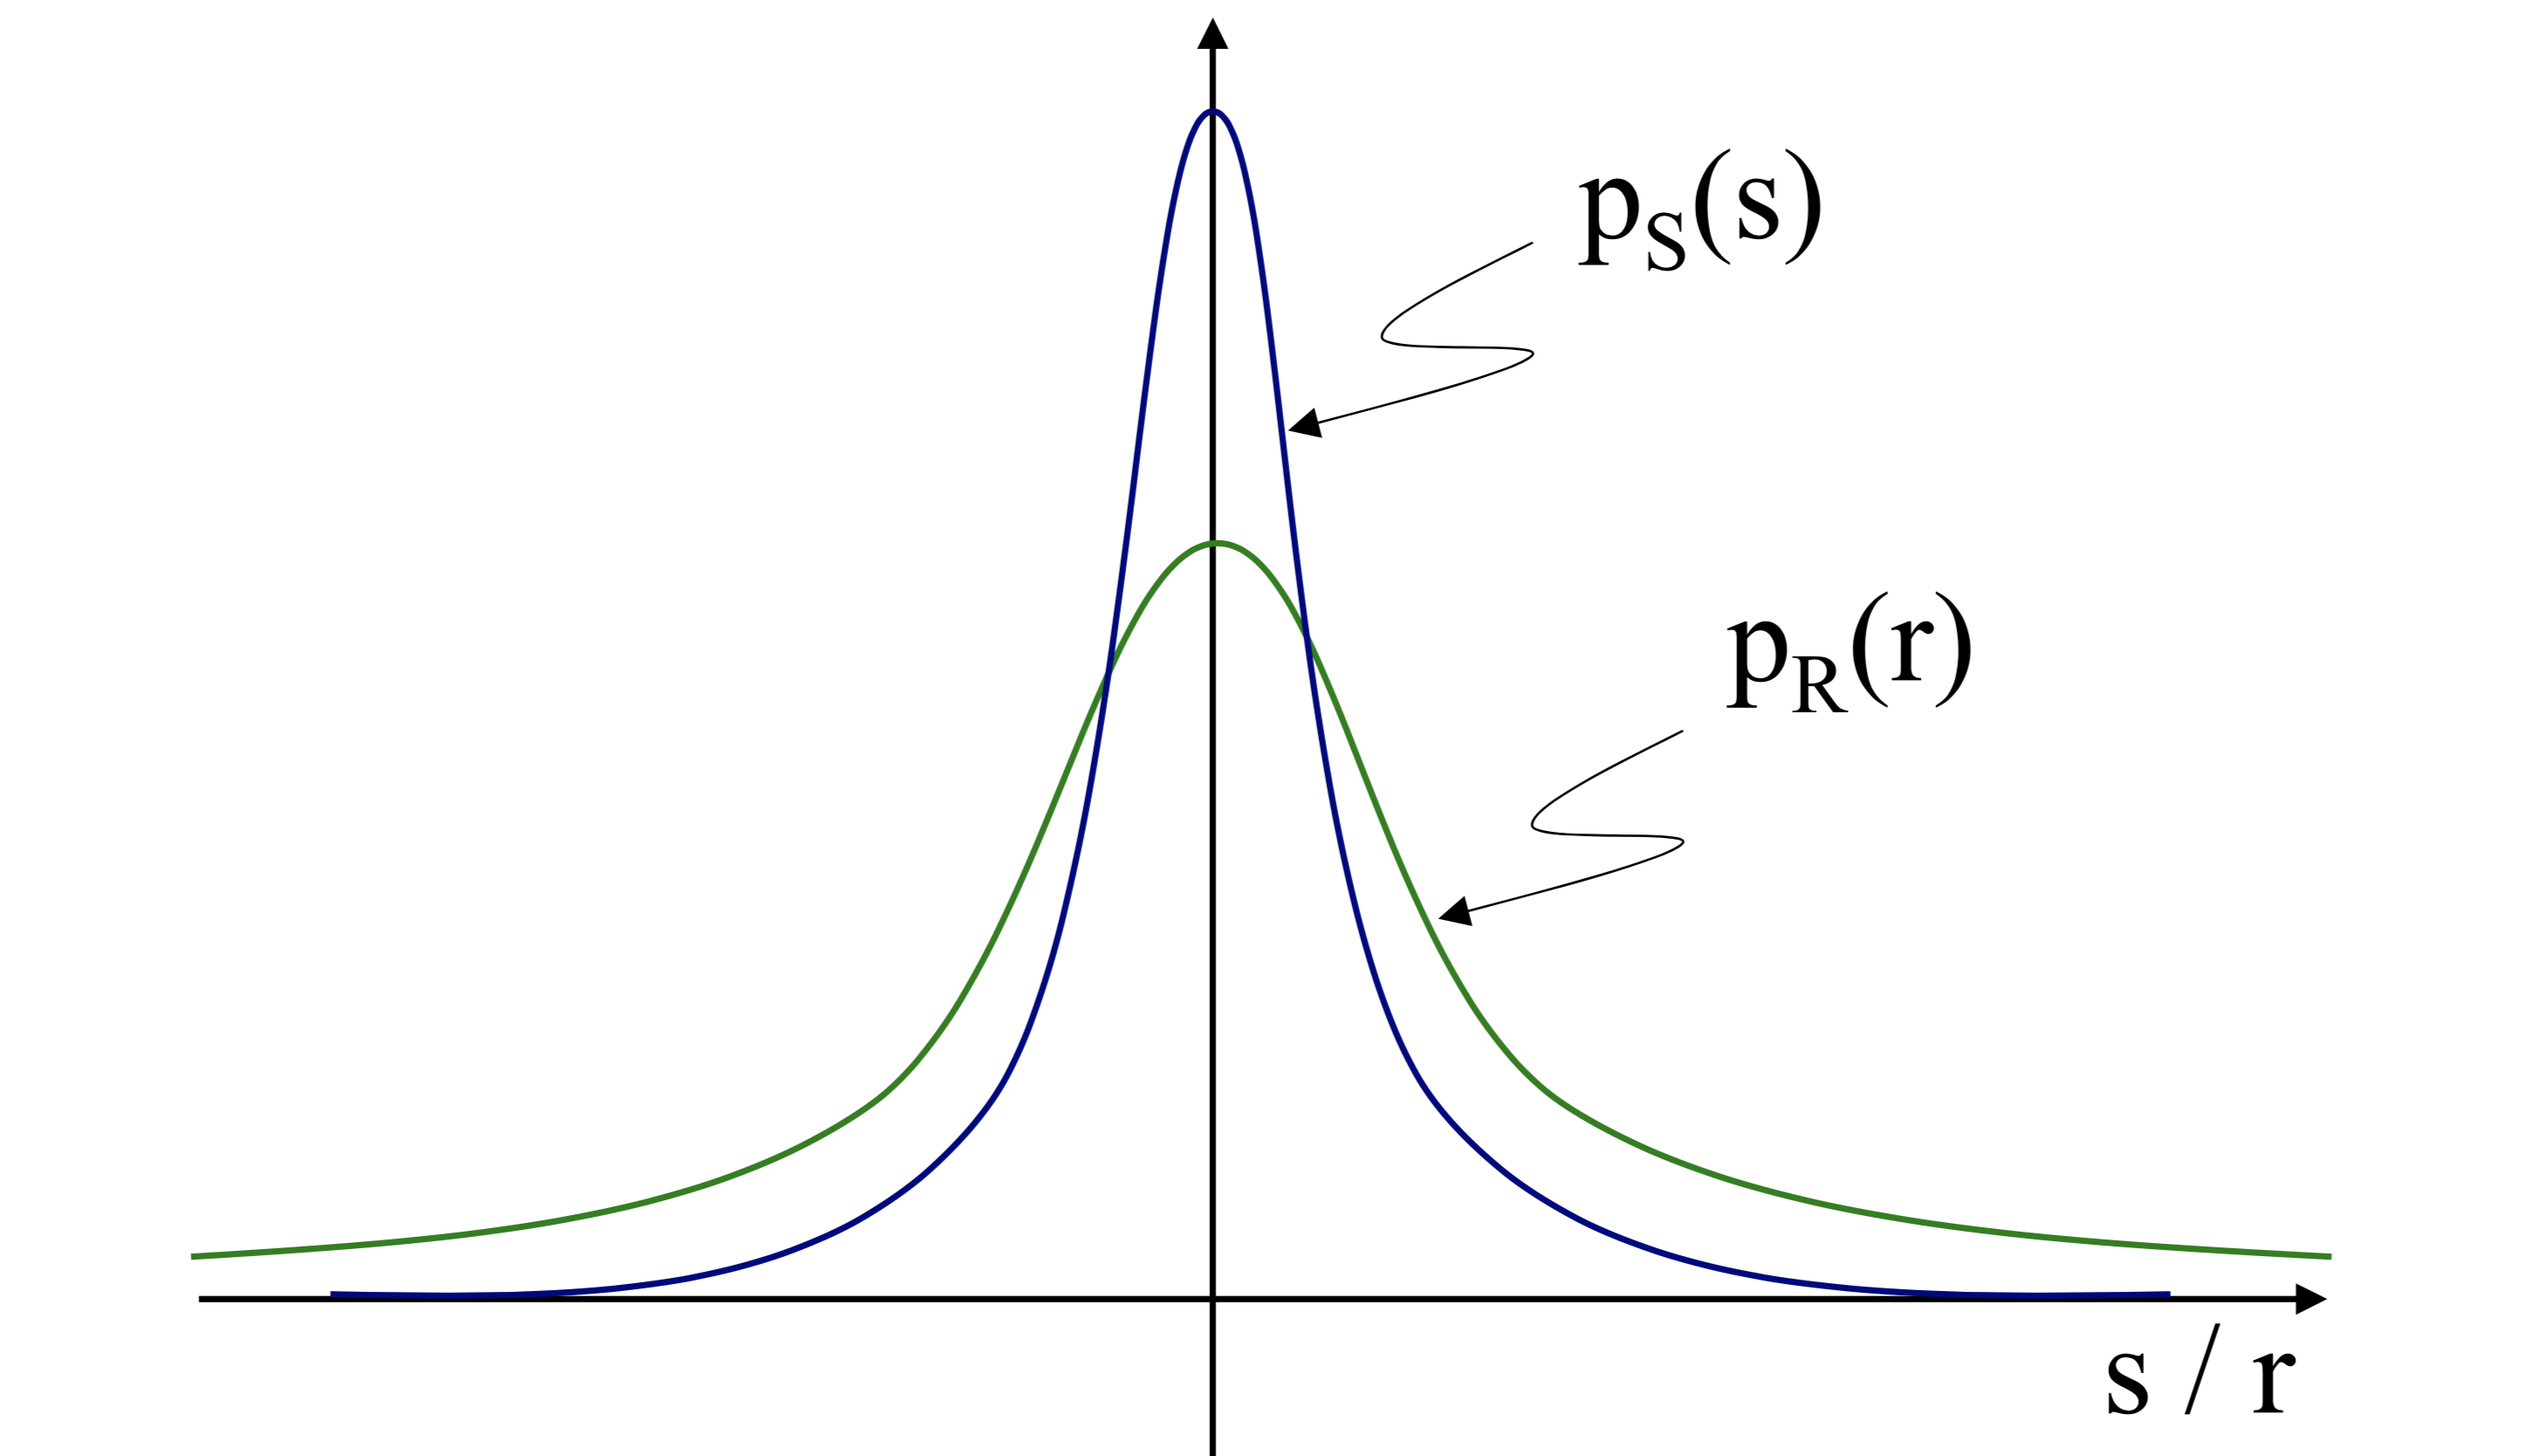
\includegraphics[width=7cm]{Figures//estimacion_caso_gauss.png}
    \caption{Estimation of Gaussian random variable $S$ contaminated by Gaussian noise $R$.}
    \label{fig:estimacion_caso_gauss}
  \end{center}
\end{figure}

According to \eqref{ec_estimador_caso_gaussiano_final}, for the resolution of the problem we must find the variance of $X$ and the covariance between $S$ and $X$ ($\rho$). The variance $v_X$ is obtained simply as the sum of $v_S$ and $v_R$ because both are independent variables. For the covariance calculation,
\begin{equation}
\rho = \mathbb{E} \{(X-m_X)(S-m_S)\} = \mathbb{E} \{X\;S\} = \mathbb{E} \{(S + R) S\} = \mathbb{E} \{S^2\} + \mathbb{E} \{S\;R\} = v_S
\end{equation}
where independence of $S$ and $R$ has been used, and the fact that all variables (including $X$) have zero means.

Replacing these results in \eqref{ec_estimador_caso_gaussiano_final} we get
\begin{equation}
\hat s_{\text{MSE}} = \frac{v_S}{v_S + v_R} x
\end{equation}

This result can be interpreted quite intuitively: when the variance of the noise is much lower than that of the signal (high Signal to Noise Ratio (SNR), $v_S \gg v_R$) we get $\hat s_{\text{MSE}} \to x$, which makes sense since the effect of the noise component in this case is not very significant; on the contrary, when the SNR is very small ($v_S \ll v_R$), the observation barely provides information about the $S$ value in each experiment, so the estimator keeps the mean value of the signal component, $\sMSE \to 0$.
\end{example} %\vspace{0.4cm}
%%%%%%%%%%%%%


%%%%%%%%%%%%%%%%%%%%%%%%%%%%%%%%%%%%%%%%%%%%%%%%%%
\subsection{Case with multidimensional variables}

{In a general multidimensional case, ${\bf S}$ and ${\bf X}$ can be random vectors of dimensions $N$ and $M$, respectively, with joint Gaussian distribution.
\begin{equation}
p_{{\bf S},{\bf X}}({\bf s},{\bf x}) 
   \sim G\left(\left[\begin{array}{c} {\bf m_S} \\ {\bf m_X} \end{array}\right],
               \left[\begin{array}{cc} {\bf V_S}          & {\bf V_{SX}}   \\ 
                                       {\bf V}_{\bf SX}^T & {\bf V_{X}}   
                     \end{array}\right]\right)
\end{equation}
being ${\bf m_S}$ and ${\bf m_X}$ the means of $ {\bf S}$ and $ {\bf X}$, respectively, ${\bf V_S}$ and ${\bf V_X}$ the covariance matrix of ${\bf S}$ and  ${\bf X}$, respectively, and ${\bf V_{SX}}$ the matrix of crossed covariances of ${\bf S}$ and ${\bf X}$, that is,
\begin{align}
{\bf V_S} &= \mathbb{E}\{({\bf S}-{\bf m_S})({\bf S}-{\bf m_S})^\intercal\} \\
{\bf V_X} &= \mathbb{E}\{({\bf X}-{\bf m_X})({\bf X}-{\bf m_X})^\intercal\} \\
{\bf V_{SX}} &= \mathbb{E}\{({\bf S}-{\bf m_S})({\bf X}-{\bf m_X})^\intercal\}
\end{align}
%La expresión general de la densidad de probabilidad es, por tanto
%\begin{align}
%p_{{\bf S},{\bf X}}({\bf s},{\bf x}) 
%   & = \frac{1}
%            {(2\pi)^{(M+N)/2} 
%             \left|\left[\begin{array}{cc} 
%                          {\bf V_S}    & {\bf V_{SX}}   \\ 
%                          {\bf V}_{\bf SX}^T & {\bf V_{X}} 
%                         \end{array}\right]
%             \right|^{1/2}} \times \nonumber\\
%    &  \times\exp\left[-\frac{1}{2}
%                  \left[\begin{array}{c} {\bf s}-{\bf m_S} \\ {\bf x}-{\bf m_X} \end{array}\right]^T                       
%                  \left[\begin{array}{cc} 
%                           {\bf V_S}          & {\bf V_{SX}} \\ 
%                           {\bf V}_{\bf SX}^T & {\bf V_{X}} 
%                        \end{array}\right]^{-1}
%                  \left[\begin{array}{c} {\bf s} \\ {\bf x} \end{array}\right]
%       \right]
%\end{align}
%La distribución a posteriori de $S$ se puede obtener como:
%\begin{align}
%p_{{\bf S}|{\bf X}}({\bf s}|{\bf x}) 
%   & = \frac{p_{{\bf S},{\bf X}}(s,x)}{p_{\bf X}(x)} \nonumber\\
%   & = \frac{(2\pi)^{M/2}|{\bf V}_{\bf X}|^{1/2}}
%            {(2\pi)^{(M+N)/2} 
%             \left| \left[\begin{array}{cc} 
%                             {\bf V_S}    & {\bf V_{SX}}   \\ 
%                           {\bf V}_{\bf SX}^T & {\bf V_{X}} 
%                    \end{array}\right]
%                    \right|^{1/2}} \times \nonumber\\
%    &  \times\exp\left[-\frac{1}{2}
%                  \left[\begin{array}{c} {\bf s} \\ {\bf x} \end{array}\right]^T                       
%                  \left[\begin{array}{cc} 
%                           {\bf V_S}          & {\bf V_{SX}} \\ 
%                           {\bf V}_{\bf SX}^T & {\bf V_{X}} 
%                        \end{array}\right]^{-1}
%                  \left[\begin{array}{c} {\bf s} \\ {\bf x} \end{array}\right]
%                 -\frac{1}{2} {\bf x}^T{\bf V_X}^{-1}{\bf x} \right]
%\end{align}

The calculation of the posterior distribution of ${\bf S}$ given ${\bf X}$ is more complex than in the one-dimensional case, but it follows a similar procedure, which we will omit here. It can be shown that the posterior distribution is Gaussian with mean
\begin{align}
{\bf m}_{{\bf S}|{\bf X}} 
      = {\bf m}_{\bf S} + {\bf V}_{\bf SX}{\bf V_X}^{-1}({\bf x}-{\bf m}_{\bf X}) 
\label{Est:sMMSEgaussMN}
\end{align}
and covariance
\begin{align}
{\bf V}_{{\bf S}|{\bf X}} 
      = {\bf V_S}- {\bf V}_{\bf SX}{\bf V_X}^{-1}{\bf V}_{\bf SX}^T
\end{align}
Since the minimum MSE estimator of ${\bf S}$ given ${\bf X}$ is precisely the posterior mean, we can write
\begin{framed}
\begin{align}
\hat{\bf s}_{\text{MSE}} = \hat{\bf s}_{\text{MAD}} = \hat{\bf s}_{\text{MAP}} = 
{\bf m}_{{\bf S}|{\bf X}} = {\bf m}_{\bf S} + {\bf V}_{\bf SX}{\bf V_X}^{-1}({\bf x}-{\bf m}_{\bf X}) 
\label{Est:sMMSEgaussGral}
\end{align}
\end{framed}
%This estimator expression is simplified when ${\bf S}$ and ${\bf X}$ have zero means, resulting in
%\begin{align}
%\hat{\bf s}_{\text{MSE}} = {\bf m}_{{\bf S}|{\bf X}} 
%      = {\bf V}_{\bf SX}{\bf V_X}^{-1}{\bf x} 
%      \label{Est:sMMSEgaussMN0}
%\end{align}}
%Partiendo de \eqref{Est:sMMSEgaussMN0} pueden obtenerse diversos casos particulares de interés en aplicaciones prácticas del procesado de señales. Algunos de ellos se analizan en el Apéndice \ref{Sec:Est:CasosGauss}.

%%%%%%%%%%%%%%%%%%%%%%%%%%%%%%%%%%%%%%%%%%%%%%%%%%%%%%
\subsection{Linear estimation and Gaussian estimation}

{Note that, if the target variable is scalar, \eqref{Est:sMMSEgaussGral} is identical to \eqref{Est:slmse}. This is not coincidental: if the minimum MSE estimator in the Gaussian case is linear, it must be equal to the best linear estimator, which is given by \eqref{Est:sMMSEgaussGral}.}

%Regrouping the terms of \eqref{Est:sMMSEgaussGral}, we can express $\hat{\bf s}_{\text{MSE}}$ as:
%\begin{framed}
%\begin{align}
%\hat{\bf s}_{\text{MSE}} = ({\bf m}_{\bf S} - {\bf V}_{\bf SX}{\bf V_X}^{-1}{\bf m}_{\bf X} )+ {\bf V}_{\bf SX}{\bf V_X}^{-1}{\bf x} 
%\end{align}
%\end{framed}
%and identifying these terms with the coefficients of a linear estimator, we get
%\begin{align} 
%{\bf w}^T =  {\bf V}_{\bf SX}{\bf V_X}^{-1}
%\end{align}
%\begin{align} 
%w_0 = {\bf m}_{\bf S} - {\bf w}^T {\bf m}_{\bf X}
%\end{align}
%These expressions align with the alternative solution of the linear estimation of mean squared error (equations \ref{ec:solucionw0} and  \ref{ec:solucionw}). This is not surprising: since the unrestricted MSE estimator in the Gaussian case is linear, the best linear estimator must match the one obtained for the Gaussian case.

%Obsérvese, por último, que \eqref{ec:solucionw} asume que {${\bf V}_{\bf X}$} es una matriz no singular. La invertibilidad de {${\bf V}_{\bf X}$} implica que ninguna componente de ${\bf X}$ puede obtenerse como combinación lineal del resto de componentes. Cuando esto no es así, puede comprobarse que la solución al problema de minimización no es única, y por lo tanto conviene eliminar las variables redundantes antes de proceder al diseño del estimador.

